\section{Methodology}\label{sec:methodology}
We build on the technique proposed by Halderman (ref to the initial paper that
proposed this).
\textbf{ discuss basic idea of the approach and add a summary of shortcomings
of that approach; what practicalities does it ignore?} 

\subsection{Dealing with Multiple Paths}
Because load-balancers can affect our measurements and conclusions, we fix the
paths our probes take in the following fashion (in line with the literature):
\begin{itemize}
    \item For ICMP:
    \item For DNS:
    \item For TCP/HTTP:
\end{itemize}
\textbf{Do our probes across different protocols take wildly different paths?
We need some validation on this, and may need a strategy to identify and filter
the cases that do not.}

We sampled a set of 1000 domains from Alexa top 1M list. This sample was resolved from three vantage points Turkey, USA and Russia, and the resulting ip addresses were traceroute using TCP, ICMP and HTTP protocols, using an upper hop count threshold of 25. (All of these measurements were already completed previously)
Using our custom analysis script, the common webservers across the vantage points and their corresponding traceroutes were then extracted and the rest of the data was discarded. This resulted in 504 common webservers. Then another level of filtering was applied, which was to only consider those webservers for which we received a reply and that to from the server in question, for all of the three protocols.
This resulted in vantage point specific filtered list, due to our 25 hop threshold, not every common webserver in the list was reachable from all the vantage points. Therefore, for each list we computed for how many webservers the path lengths of protocol X and Y are exactly same: for example, X=ICMP and Y=TCP path length were exactly same (labeled as ICMP-TCP in Table~\ref{tab:samepathvalidation}) for Russia, 206 times out of 296 successful traceroutes. The last column represents count of same path length for all three protocols combined.

From a high level view, Table~\ref{tab:samepathvalidation} represents ICMP and HTTP path lengths differ more as compared to ICMP-TCP or HTTP-TCP. The difference in HTTP-TCP path length is mostly due to receiving RST packets from the server during HTTP traceroute, which would terminate it prematurely. Same logic is applicable for ICMP-TCP path lengths being more similar (having a higher count in table) than the ICMP-HTTP path lengths. On average ~65\% of the times all three protocol path lengths were exactly same, according to the last column of the table.

\subsection{Reference (ICMP) Path Validation}
\begin{itemize}
    \item So and so papers have shown that routers and servers can block ICMP
        probes.  We first establish the rate of such blocking (manifested by
        incomplete paths).
     \item Experiment: For a sample of top Alexa websites (10K), check
         reachability (path completeness and path inflation) to their
         authoritative name-servers and webservers over ICMP.  
     \item \textit{Path inflation:} Mention how we discover it: we started with
         TTL of 25 and were getting a high percentage of incomplete paths.
         Increasing the TTL to 64, increases the coverage of complete paths,
         but inflates it.
     \item Show empirical results and build an argument for discarding
         incomplete and inflated paths.
     \item Confirm that this happens from all vantage points.
\end{itemize}

\subsection{Path Validation Data Collection}
We decided to use Alexa Top 1M list, and randomly selected top 1000 domains from 100000 top domains. We did this to ensure that our current sample has sufficient variability with respect to where the servers are hosted, and who these servers belong to. For example, there a lot of www.google.** domains in top Alexa domains.


We firstly resolve those 1000 domains using a custom resolver code[Link code's repo]. We used, this custom script and not the local resolver to make sure that the authoritative server of that domain replies to our IP rather than our local resolver's IP which move out of our domain of control. So this step was taken to ensure repeatability. This resolver code takes in a list of of domains and returns a file which has data in the following format. \\ 
\begin{center}
   domain, cname, authserverIP, webserverIP \\    
\end{center}
We then divide the list into two sets, one set contains the list of domain and its corresponding authserverIP and the second set contains the list of domain and its corresponding webserverIP. We currently have rented four servers located at following locations: \\
1. USA\\
2. Russia\\
3. Turkey\\
4. China\\

Unfortunately we were unable to run any measurement beyond resolution on Chinese machine primarily because its a CentOS machine and we had to recompile a lot of scripts for that particular environment. With that said, we were able to resolve and run measurements from those three vantage points and collect data. 

We ran a couple of preliminary measurements and found out that a lot of ICMP probes were not reaching the server, so our primary hypothesis was that most of the path were getting inflated because of IDS. So proposed way to measure this was to send ICMP packets with a higher TTL value so that IDS cases get eliminated and we have a solid set of paths onto which we can base our methodology. 


So in this experiment, as mentioned earlier we would run two different set of traceroutes on different sets of resolved servers. For the Authoritative server we will send ICMP and UDP (DNS packets with query to get current bind version) probes. For Webservers we will send ICMP, TCP and HTTP packets. We set the intial max TTL value to be default traceroute value which is 25, and then we collected the results and analyzed them and then ran the same experiment with max TTL value of 64. For both the experiments if we do not receive a response for 15 consecutive hops, we terminate the traceroute.

We made a couple of assumptions in our analysis, first of all we assumed was in path inflation code. We assumed that if there are more than two non responding consecutive IPs in the traceroute we assumed that the path is inflated because of IDS. 

Secondly, we are assuming that if there is no reply for fifteen consecutive hops then the server will not respond for the max ttl value either. Which essentially implies that IDS is completely blocking our access.

Before we go into the analyzing the results, we will first enlist the base numbers to give weight to the percentages. \\

In Russia there were a total of 805 unique webserver, and 869 unique authservers.
In USA there were a total of 793 unique webserver, and 871 unique authservers.
In Turkey there were a total of 788 unique webserver, and 867 unique authservers.


On a very high level, the results show a difference in percentage of ICMP probes that reach the server. On average around 85 percent of ICMP probes with TTL 25, and 98 percent ICMP probes when TTL value is 64, reach authoritative servers. Similarly, for in case of webservers we saw roughly equal reach-ability of about 75 percent for both 25 and 64 TTL. 

There was a significantly higher path length inflation in ICMP paths to authservers compared to webservers (average of 25 percent vs 10 percent). 

Broadly speaking, the TTL configuration of 64 with 15 gap limit would be ideal way to probe both webservers and authoritative servers, however there is a much higher incidence of ICMP blocking around webservers compared to authservers. In worst case we would be dropping around 20 percent of ICMP probes (if we dont fix the path inflation) for webservers and around 35 percent in case of authservers.

\begin{table*}
\small

    \begin{center}

    \begin{tabular}{|l|r|r|r|r|r|r|r|r|} \hline
        \multirow{4}*{Vantage Point} &
        \multicolumn{4}{c|}{Authoritative Nameservers Reachability} 
         &
        \multicolumn{4}{c|}{Webservers Reachability}
         \\ \cline{2-9}
        & 
        \multicolumn{2}{c|}{\% Complete Paths} 
        &
        \multicolumn{2}{c|}{\% Possible Inflated Paths}
        &
        \multicolumn{2}{c|}{\% Complete Paths} 
        &
        \multicolumn{2}{c|}{\% Possible Inflated Paths}
        \\ \cline{2-9}



        & \multirow{2}*{TTL=25} &
          \multirow{2}*{TTL=64} &
          \multirow{2}*{TTL=25} &
          \multirow{2}*{TTL=64} &
          \multirow{2}*{TTL=25} &
          \multirow{2}*{TTL=64} &
          \multirow{2}*{TTL=25} &
          \multirow{2}*{TTL=64} 

                        \\ 
                        
        &&&&&&&& \\  \hline

        Russia
        & 87.2 & 98.3 & 23.2 & 23.5 & 75.1 & 75.8 & 10.7 & 11.1
             \\ \hline

        Turkey
        & 84.3 & 99.5 & 33.2 & 36.5 & 75.6 & 78.0 & 9.9 & 11.9 
             \\ \hline

        USA
        & 84.7 & 98.6 & 22.8 & 25.1 & 73.7 & 76.5 & 7.1 & 9.5
             \\ \hline
        
        China
        & NA & NA & NA & NA & NA & NA & NA & NA
             \\ \hline

    \end{tabular}

    \caption{ICMP reachability for Y websites. We start with the
        Alexa top 10,000.  Filter down to the set that have the same
        authoritative name server from all vantage points, resulting in n =  X.
        We further filter down to the set that have the same webserver across
    all vantage points, resulting in n = Y.}
    \label{tab:pathvalidation}

    \end{center}
\end{table*}


\begin{table*}
\small

    \begin{center}

    \begin{tabular}{|l|r|r|} \hline
        Number of Vantage Points &
        Authoritative Nameservers 
        (n=) &
        Webservers
        (n=)

        \\ \hline

        None    & 72 & 170 \\ \hline
        Only one & 3 & 4 \\ \hline
        Only two & 8 & 8 \\ \hline
        All Three & 437 & 383 \\ \hline
       
       
    \end{tabular}

    \caption{ICMP reachability for Y websites using three back-to-back ICMP
        probes (TTL = 64). We start with the
        Alexa top 1,000.  Filter down to the set that have the same
        authoritative name server from all vantage points, resulting in n =  X.
        We further filter down to the set that have the same webserver across
    all vantage points, resulting in n = Y.}
    \label{tab:ICMPreachabilityacrossvantages}

    \end{center}
    X=520\\
    Y=565
    
\end{table*}

From a high level view, the data shows that there were roughly half the number of vantage points who had same server replying to all the vantage points, this counters the previously made assumption regarding the prevalence of CDNs in the list (at least for the vantage points we currently have). With that said, there was a roughly equal number of servers that were doing some degree of ICMP blocking based on the geo-location 11 in Authservers and 12 in Webservers. The non replying servers across the VPs suggest that we have ICMP blocking implemented at those servers and they should be filtered before we start our actual measurement phase.

While analyzing the IPs reachable from one or two vantage points, first major observation was that these IPs were reachable using traceroutes and not using ZMap. This is counter-intuitive because scamper's probes are under more restrictions compared to ZMap's probes (15 gap limit). The second major observation was that even for some cases even if the ICMP probes were not reaching the end host, the TCP probes were reaching the end host. Specifically in case of russian vantage point, in which the TCP packets were getting intercepted by a server close by (6th hop from the VP) and the ICMP probes were reaching on average thirteen hops before getting lost in the abyss. 

\begin{table*}
\small

    \begin{center}

    \begin{tabular}{|l|r|r|r|r|} \hline
        \multirow{2}*{Vantage Point} &
        \multicolumn{4}{c|}{Common Webservers across VPs - Path Length Analysis (Y)}
         \\ \cline{2-5}
        & ICMP-TCP &
          HTTP-TCP &
          ICMP-HTTP &
          ICMP-HTTP-TCP\\ \hline
                        
        Russia ($Z_{r}$=296)
        & 206 & 236 & 178 & 172   
             \\ \hline

        Turkey ($Z_{t}$=269)
        & 227 & 221 & 192 & 190 
             \\ \hline

        USA ($Z_{u}$=281) 
        & 225 & 245 & 199 & 197 
             \\ \hline

    \end{tabular}

    \caption{Started with a random sample of
        Alexa 1000. Filtered down to the set that have the same webservers from all vantage points resulting in n = Y. Further filtered down the set of webservers for which the server in question replied, for all protocols, resulting in $Z_{i}$, specific to each vantage point. Protocol A - Protocol B label represents the number of traceroutes which have same path length, in Y, for both protocol A and protocol B.}
    \label{tab:samepathvalidation}

    \end{center}
    Y = 504\\
\end{table*}

\begin{figure*}[!h]
\centering
  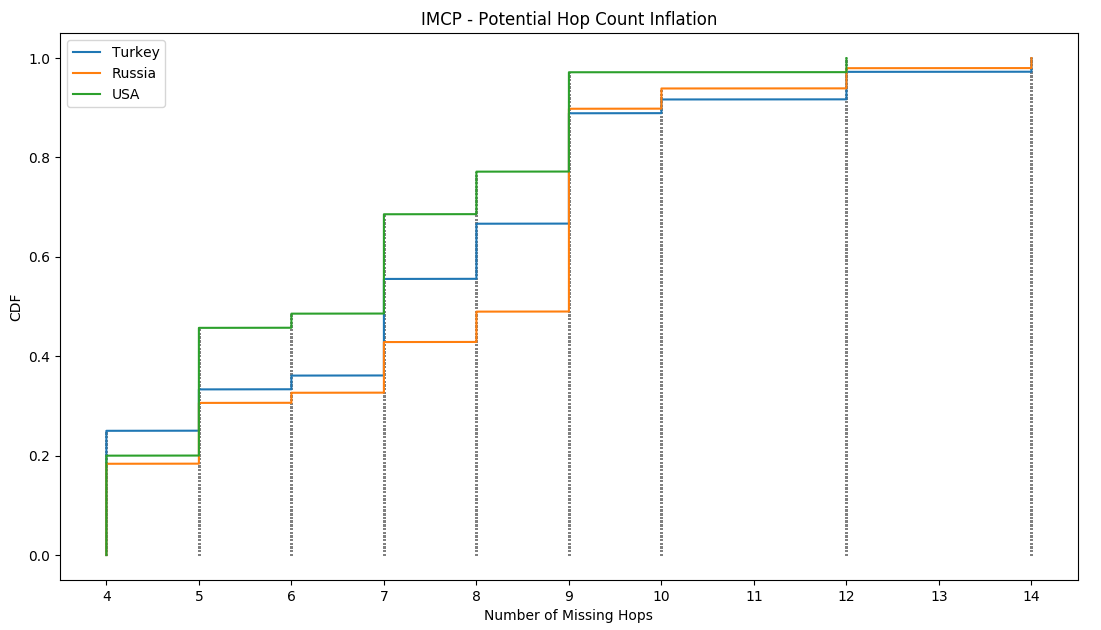
\includegraphics[width=\linewidth]{figures/missing-hops-cdf.png}
  \caption{Distribution of path length inflation at \textit{n} non-responding hops for 504 common webservers across all vantage points.}
  \label{fig:inflated-path-cdf}
\end{figure*}

\subsection{Inflated Paths - Missing hops}
Figure~\ref{fig:inflated-path-cdf} shows the distribution of inflated paths for ICMP traceroutes that appear complete (we can reach server in question), but responses between hops are missing. The analysis has been carried on the list of webservers that were common for all vantage points.

The results significantly vary among the vantage points due to the differences in path length in reaching the same server. For example, if a webserver 'X' is 8 hops away from our vantage point in Russia and 12 hops away from our vantage point in USA. And an IDS is situated on path to the server which does not allow packets with lower than 14 ttl value to pass, then traceroute from Russia  will have 6 missing hops whereas traceroute from USA will have 2 missing hop, for the same webserver. This variance in path length is contributing towards the variation in CDF across vantage points.
